\documentclass[11pt]{article}
\usepackage[a4paper,margin=1in]{geometry}
\usepackage{mathtools, amsthm, amssymb, amsmath}
\usepackage{multicol}

\usepackage[style=numeric, sorting=none]{biblatex}
\addbibresource{MV.bib}

\usepackage{graphicx}
\graphicspath{{./picture/}}

\usepackage{tikz}
\usetikzlibrary{positioning}

\usepackage{rotating}

\newtheorem{definition}{Definition}
\newtheorem{example}{Example}

\title{Generating of Music Variations: Dynamical Systems Approach}
\author{Rajamangala University of Technology Thanyaburi\\Kanatsanun Sub-udom\\Wannasa Rianthong\\Patipan Somwong}

\begin{document}

\section{Literature Review}

\subsection{Fourth-Order Runge–Kutta Method}
While analytical solutions exist for some differential equations, many require numerical approaches to approximate their behavior. The field of mathematics offers a numerical methods for solving both single and systems of linear and nonlinear differential equations. Popular examples include the Euler method and Taylor series methods. However, when it comes to achieving a balance between accuracy and efficiency, the Runge-Kutta method reigns supreme for approximating solutions.

The Runge-Kutta method \cite{bose_numerical_2019} is a numerical methods for approximating solutions to ordinary differential equations. These equations describe how a quantity changes with respect to another variable, but often cannot be solved exactly. The Runge-Kutta method tackles these problems by breaking down the interval of interest into smaller subintervals and iteratively calculating the solution at each subinterval. 

\subsection{Melodic Variation}

Let $\dot{y} = f(t,y)$. The approximation of $y_{i+1}$ by fourth-order Runge–Kutta method is given by:
\begin{align*}
y_{i+1} &= y_i + \dfrac{h}{6}(k_1 + 2k_2 + 2k_3 + k_4), \\
k_1 &= f(t_i, y_i), \\
k_2 &= f\left( t_i + \dfrac{h}{2}, y_i + \dfrac{h}{2}k_1 \right), \\
k_3 &= f\left( t_i + \dfrac{h}{2}, y_i + \dfrac{h}{2}k_2 \right), \\
k_4 &= f(t_i + h, y_i + hk_3),
\end{align*}
\label{fig:RK4}
where $i = 0,1,2,...$ and $h$ is the step size, $y$ is the variable and $t$ is time. \\
\section{Main Result}

This section explores the application of three techniques for generating musical variations, using the Ah vous dirai-je, Maman melody as a starting point and Lorenz Equation for chaotic
trajectory.

\subsection{Musical Variations from a Chaotic Mapping}

Let a sequence of pitches be represented by $P = \{p_1, p_2, \dots, p_n\}$. Let $\dot{x} = f(x)$ be a dynamical system with chaotic behavior. Then the approximate solution of $\dot{x}$ is denoted by $V = \{v_0, v_1, \dots, v_n\}$, when $v_0 \in \mathbb{R}_n$ is an initial condition of this trajectory. Let $K$ be a mapping from pitch to real value defined by 
$$K(p_i) = v_i.$$ 
Given $V^\prime = \{ v^\prime_1, v^\prime_2, \dots, v^\prime_n \}$ be a sequence of new trajectory by an initial condition of $v^\prime_0 \in \mathbb{R}_n$.

For each element $v^\prime$ in $V^\prime$, Let $L$ be a mapping from real value to pitch defines by 
$$L(v^\prime_i) = p_{j^*}.$$ 
Where $j^*$ is the chosen index for the new pitch according to the following criteria:
\begin{enumerate}
	\item If there exist the smallest $v_i$ such that $v_i > v^\prime_i$, then the new pitch must agree to use differ pitch, which is $j^* = j$ when $j$ is a index of a nearest $v_i$ value element such that $v_i > v_j$.
	\item If there exist a highest value $v^\prime_i$ such that $v_i < v^\prime_i$ for all $v_i$ in $V$, then the new pitch must agree to use highest $v_i$ value index. 
	\item If $v_i = v^\prime_j$, then the new pitch must agree to use the same pitch with the original pitch. 
	\item Otherwise, the new pitch must agree to use lowest $v_i$ value index.
\end{enumerate}
This creates a new sequence of pitches which can be represented by $\hat{P} =\{ \hat{p}_1, \hat{p}_2, \dots, \hat{p}_n \}$.

\begin{example}
Let a sequence of pitches of 12 variations on Ah vous dirai-je Maman in the first 3 bars in Figure \ref{fig:Dabby1} be represented by $P = \{C4, C4, G4, G4, A4, A4, G4, F4, F4, E4, E4 \}$. Let Lorenz system be a dynamical system with chaotic behavior by giving Lorenz parameters $r = 28, \sigma=10$ and $b = \frac{8}{3} $. Then the approximate solution of Lorenz system using fourth-order Runge–Kutta method with initial condition of $(1,1,1)$ is denoted by $X = \{1.00, 1.29, 2.13, 3.74, 6.54, 11.04, \\ 16.69, 19.56, 15.37, 7.55, 1.20\}$ when $X$ is sequence of x-value of approximate solution of Lorenz system. Let $K$ be a mapping from pitch to real value result as follows:

\begin{align*}
K(C4) &= 1.00, \\ 
K(C4) &= 1.29, \\
K(G4) &= 2.13, \\
K(G4) &= 3.74, \\
K(A4) &= 6.54, \\
K(A4) &= 11.04, \\
K(G4) &= 16.69, \\
K(F4) &= 19.56, \\
K(F4) &= 15.37, \\
K(E4) &= 7.55, \\
K(E4) &= 1.20. 
\end{align*}

Given $X^\prime = \{ 1.01, 1.30, 2.15, 3.76, 6.58, 11.10, 16.73, 19.55, 15.30, 7.48, 1.15 \}$ be a sequence of new trajectory with an initial condition of $(1.01,1,1)$ Let $L$ be a mapping from real value to pitch result as follows:
\begin{align*}
L(1.01) &= C4, \\
L(1.30) &= E4, \\
L(2.15) &= G4, \\
L(3.76) &= G4, \\
L(6.58) &= A4, \\
L(11.10) &= A4, \\
L(16.73) &= F4, \\
L(19.55) &= G4, \\
L(15.30) &= A4, \\
L(7.48) &= A4, \\
L(1.15) &= C4.
\end{align*}
This creates a new sequence of pitches which can be represented by $\hat{P} =\{C4, E4, G4, G4, A4, A4, \\ F4, G4, A4, A4, C4 \}$. Which can be converted to sheet music, as shown in Figure \ref{fig:Dabby2}. Since this method uses the same note duration and musical notes to create a new variation, so the resulting changes in the sequence compared to the original sequence might seem relatively small.
\end{example}

\begin{figure}
\centering
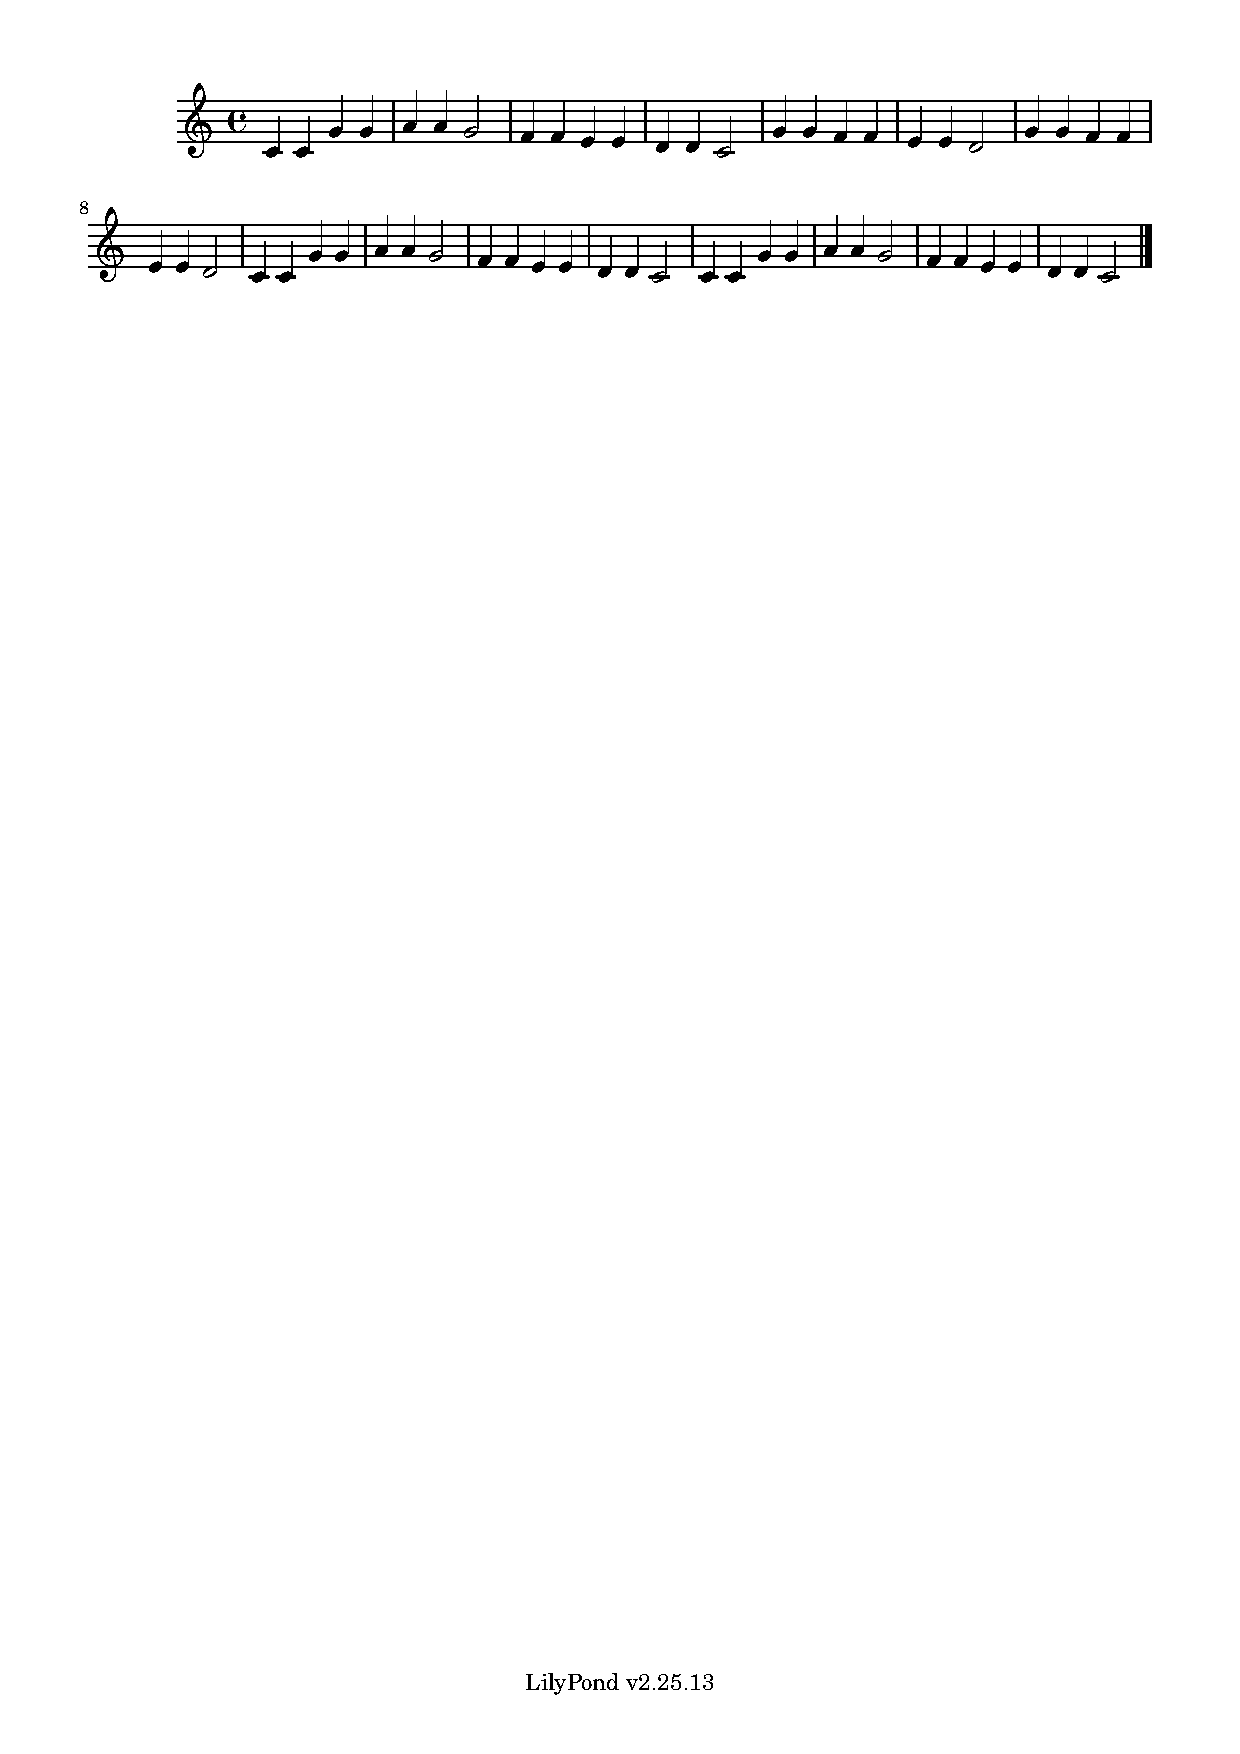
\includegraphics[trim=1cm 26.5cm 10.055cm 0.02cm, clip, scale=1]{dabby_1.pdf} % trim={left bottom right top}
\caption{The original of 12 variations on Ah vous dirai-je Maman in the first 3 bars.}
\label{fig:Dabby1} 
\end{figure}

\begin{figure}
\centering
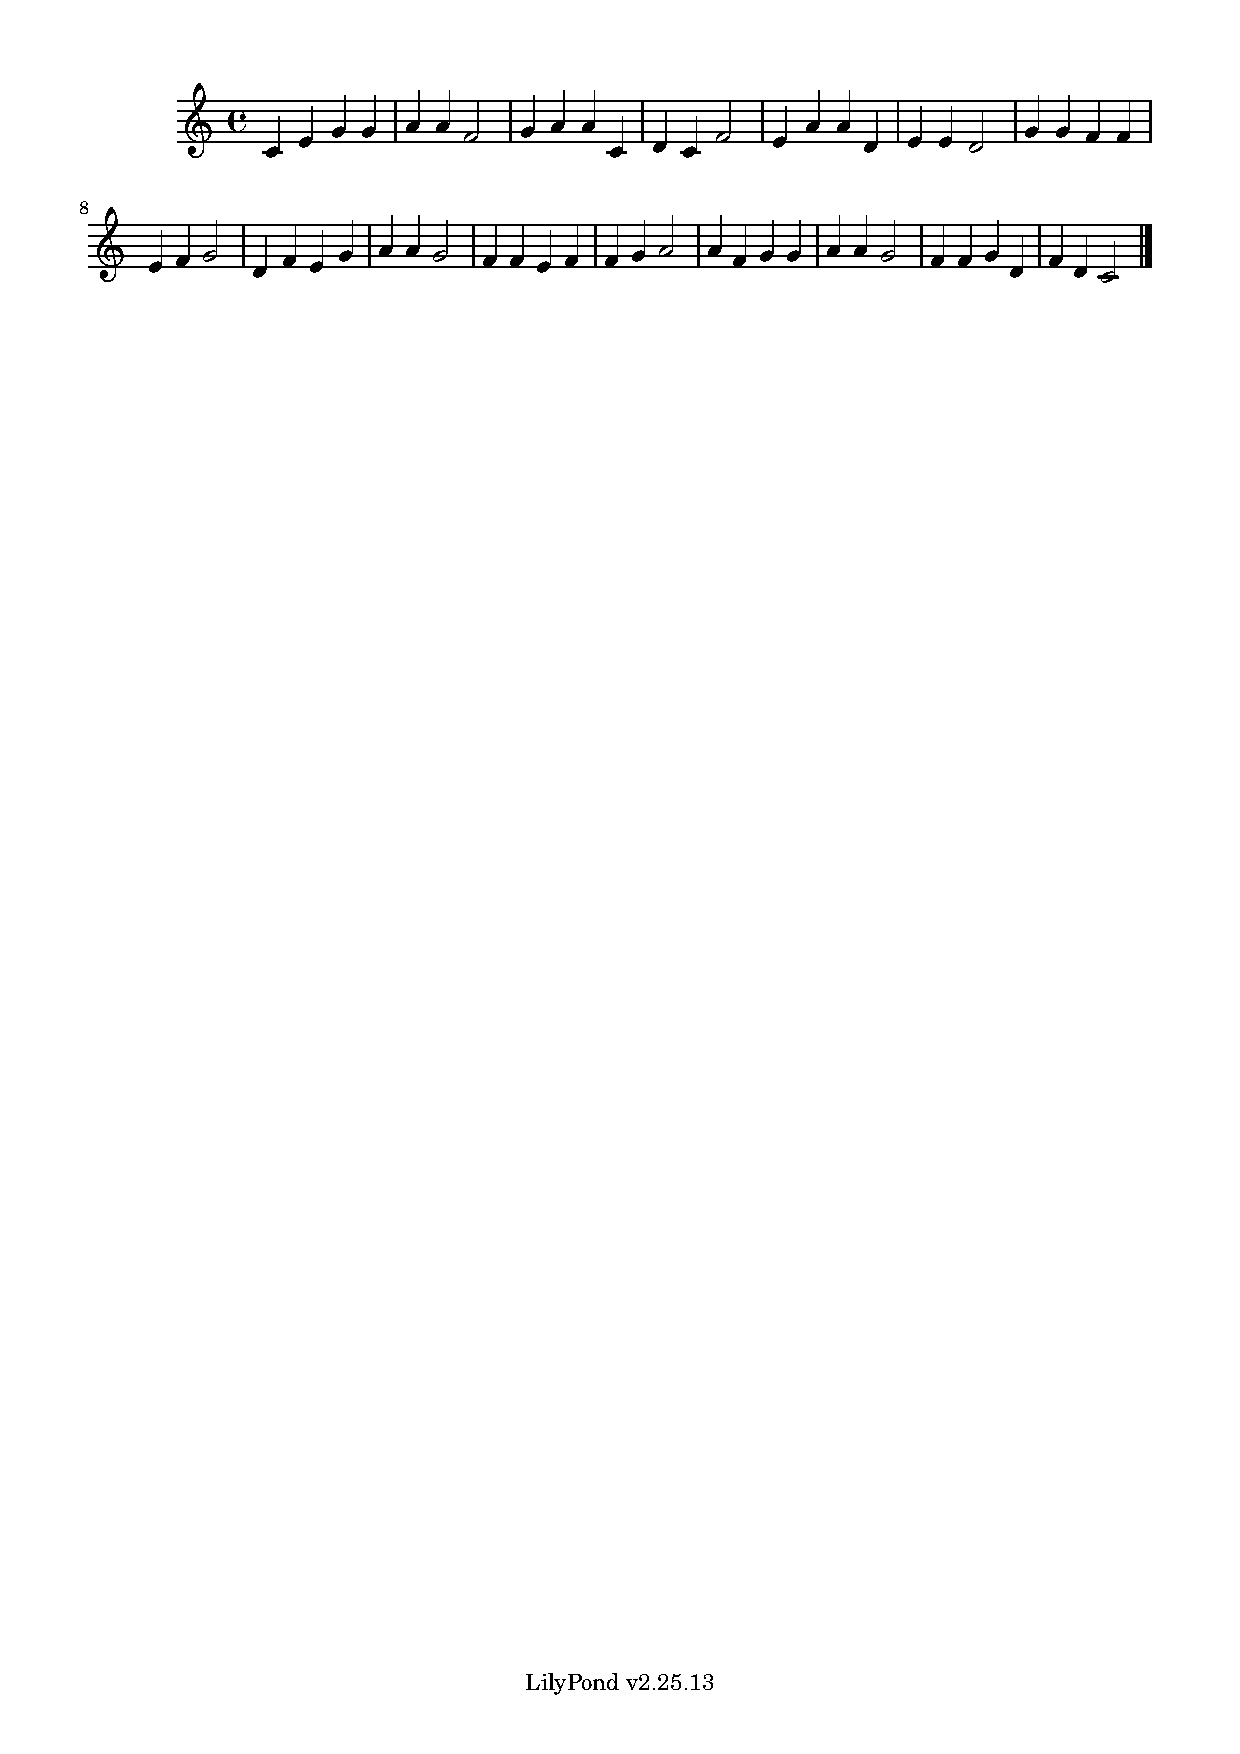
\includegraphics[trim=1cm 26.5cm 10.1cm 0.02cm, clip, scale=1]{dabby_2.pdf}
\caption{The new variation of 12 variations on Ah vous dirai-je Maman in the first 3 bars, generated by the Initial Condition $(1.01, 1, 1)$.}
\label{fig:Dabby2}
\end{figure}

\subsection{Melodic Variation with Expanded Rhythm Method} 
Given a note duration denoted by $\phi$ and divided into $D$ equal parts, the duration, $R$, of each individual division is defined by the following equation:
$$ R = \frac{\phi}{D}.  $$
\textbf{Note:} In musical theory, equal parts refers to divisions that all have the same duration.

\begin{example}
Consider the music piece 12 variations on Ah vous dirai-je Maman, illustrated in Figure \ref{fig:MV1}. The Figure shows that we already have 6 quarter notes and 1 half note.

If we want to divide each musical note into 4 parts, we can find the duration of each individual division as follows:
\begin{enumerate}
  \item[$\bullet$] Half note to 4 parts: $$R = \frac{\phi}{D} = \frac{2}{4} = 0.5$$
  \item[$\bullet$] Quarter note to 4 parts: $$R = \frac{\phi}{D} = \frac{1}{4} = 0.25$$
\end{enumerate}

Following this calculation, a half note can be divided into 4 eighth notes, and a quarter note can be divided into 4 sixteenth notes. This division is represented by the sequence \\ $P = \{C4, C4, C4, C4, C4, C4, C4, C4, G4, G4, G4, G4, G4, G4, G4, G4, A4, A4, A4, A4, A4, A4, \\ A4, A4, G4, G4, G4, G4 \}$ which can be converted to sheet music, as shown in Figure \ref{fig:MV2}.
\end{example}

\begin{figure}
\centering
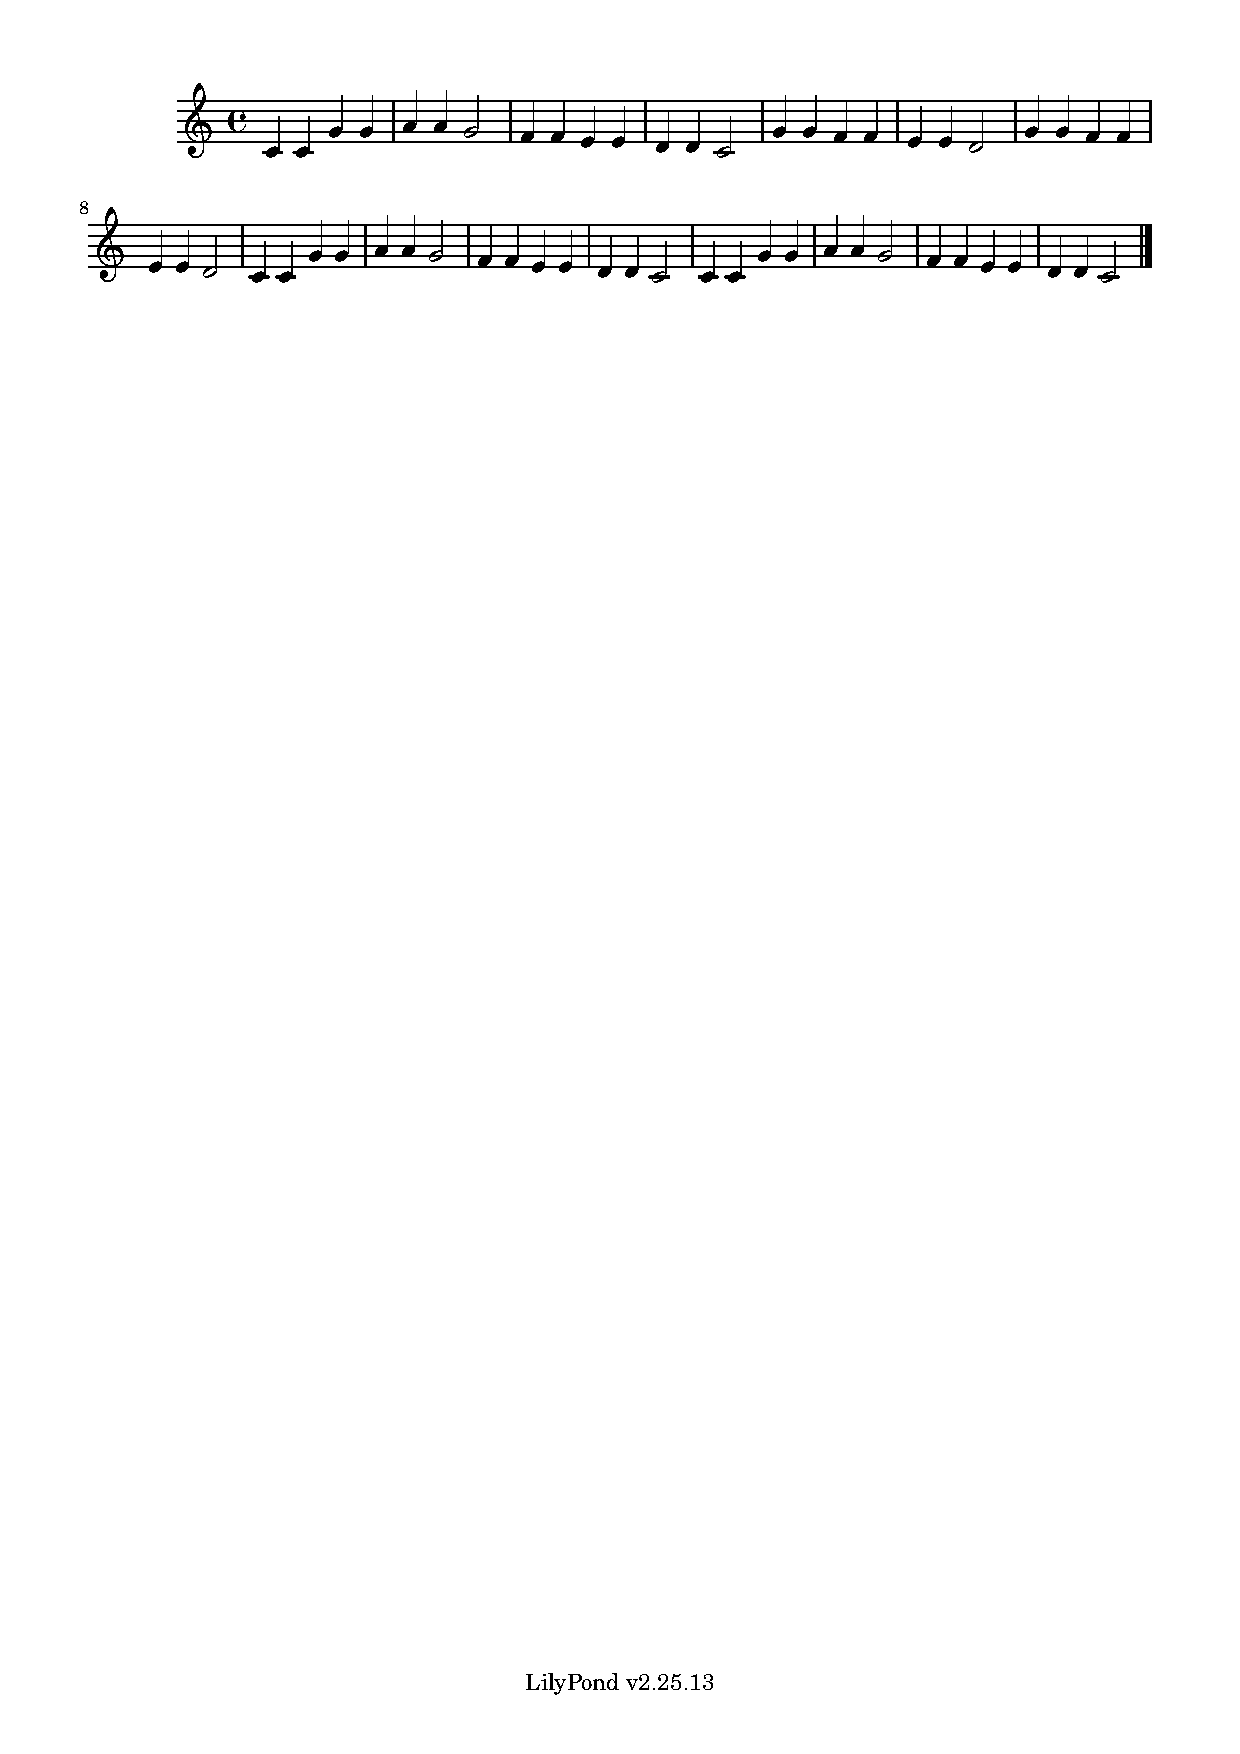
\includegraphics[trim=1cm 26.5cm 12.35cm 0.02cm, clip, scale=1]{dabby_1.pdf}
\caption{The original of 12 variations on Ah vous dirai-je Maman in the first 2 bars.}
\label{fig:MV1} 
\end{figure}

\begin{figure}
\centering
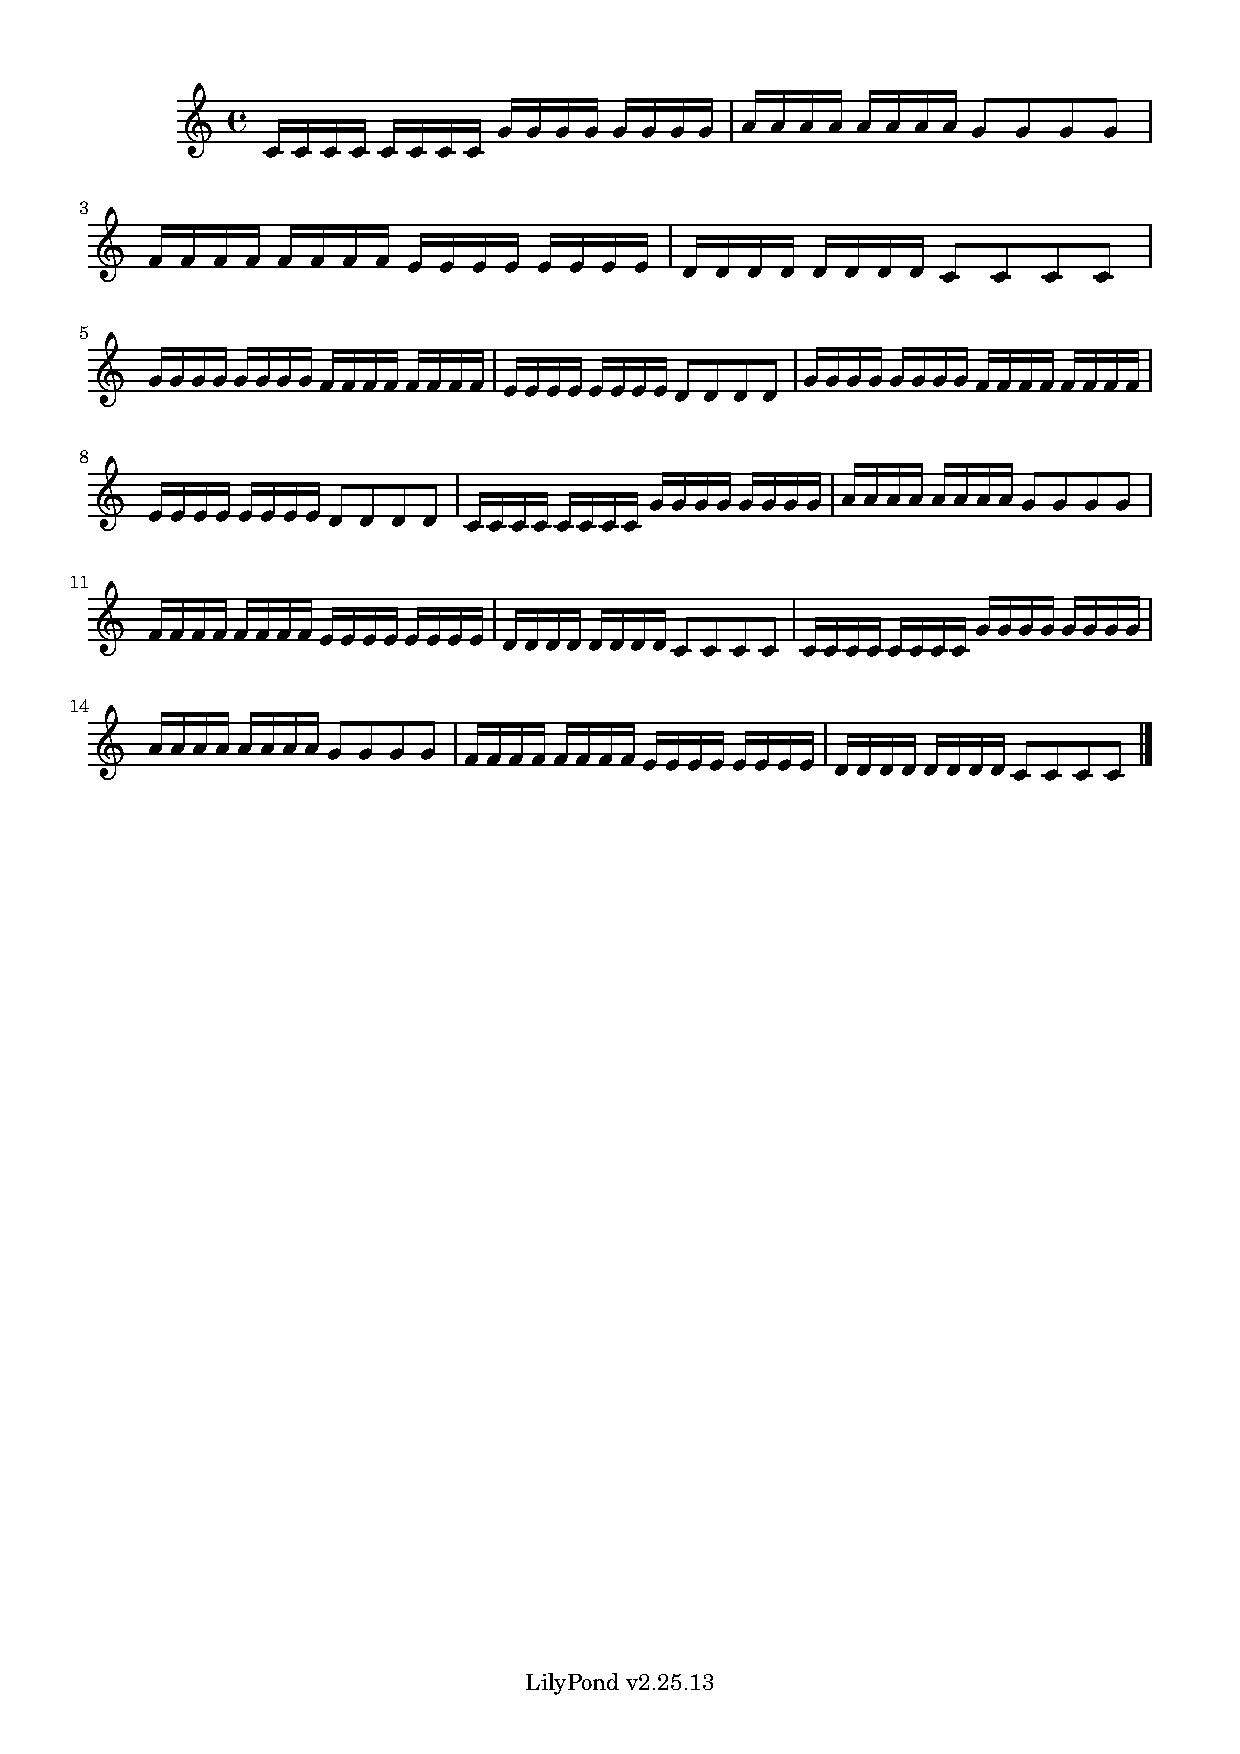
\includegraphics[trim=1cm 26.5cm 1cm 0.5cm, clip, scale=0.6]{melody_variation.pdf}
\caption{The melodic variation of Ah vous dirai-je, maman in the first 2 bars.}
\label{fig:MV2}
\end{figure}

\subsection{Combining Musical Variations from a Chaotic Mapping and Melodic Variation with Expanded Rhythm}
Let a sequence of pitches be represented by $P = \{p_1, p_2, \dots, p_n\}$ and a sequence of expanded rhythm pitches be represented by $P^* = \{p^*_1, p^*_2, \dots, p^*_n\}$. Let $\dot{x} = f(x)$ be a dynamical system with chaotic behavior. Then the approximate solution of $\dot{x}$ is denoted by $V = \{v_0, v_1, \dots, v_n\}$, when $v_0 \in \mathbb{R}_n$ is an initial condition of this trajectory. Let $K$ be a mapping from pitch to real value defined by 
$$K(p_i) = v_i.$$ 
Given $V^\prime = \{ v^\prime_1, v^\prime_2, \dots, v^\prime_n \}$ be a sequence of new trajectory with the same number of members as $P^*$ by an initial condition of $v^\prime_0 \in \mathbb{R}_n$.

For each element $v^\prime$ in $V^\prime$, Let $L$ be a mapping from real value to pitch defines by 
$$L(v^\prime_i) = p_{j^*}.$$ 
Where $j^*$ is the chosen index for the new pitch according to the following criteria:
\begin{enumerate}
	\item If there exist the smallest $v_i$ such that $v_i > v^\prime_i$, then the new pitch must agree to use differ pitch, which is $j^* = j$ when $j$ is a index of a nearest $v_i$ value element such that $v_i > v_j$.
	\item If there exist a highest value $v^\prime_i$ such that $v_i < v^\prime_i$ for all $v_i$ in $V$, then the new pitch must agree to use highest $v_i$ value index. 
	\item If $v_i = v^\prime_j$, then the new pitch must agree to use the same pitch with the original pitch. 
	\item Otherwise, the new pitch must agree to use lowest $v_i$ value index.
\end{enumerate}
This creates a new sequence of pitches which can be represented by $\hat{P} =\{ \hat{p}_1, \hat{p}_2, \dots, \hat{p}_n \}$.

\begin{example}
Let a sequence of pitches of 12 variations on Ah vous dirai-je Maman in the first 2 bars in Figure \ref{fig:MV1} be represented by $P = \{C4, C4, G4, G4, A4, A4, G4 \}$ and a sequence of expanded rhythm pitches on Figure \ref{fig:MV2} be represented by $P^* = \{C4, C4, C4, C4, C4, C4, C4, C4, G4, G4, G4, \\ G4, G4, G4, G4, G4, A4, A4, A4, A4, A4, A4, A4, A4, G4, G4, G4, G4 \}$. Let Lorenz system be a dynamical system with chaotic behavior by giving Lorenz parameters $r = 28, \sigma=10$ and $b = \frac{8}{3} $. Then the approximate solution of Lorenz system using fourth-order Runge–Kutta method with initial condition of $(1,1,1)$ is denoted by $X = \{1.00, 1.29, 2.13, 3.74, 6.54, 11.04, 16.69, 19.56, \\ 15.37, 7.55, 1.20\}$ when $X$ is sequence of x-value of approximate solution of Lorenz system. Let $K$ be a mapping from pitch to real value result as follows:

\begin{align*}
K(C4) &= 1.00, \\ 
K(C4) &= 1.29, \\
K(G4) &= 2.13, \\
K(G4) &= 3.74, \\
K(A4) &= 6.54, \\
K(A4) &= 11.04, \\
K(G4) &= 16.69.
\end{align*}

Given $X^\prime = \{1.01, 1.30, 2.15, 3.76, 6.58, 11.10, 16.73, 19.55, 15.30, 7.48, 1.15, -2.70, -4.85, \\ -6.13, -7.06, -7.87, -8.64, -9.29, -9.70, -9.73, -9.37, -8.76, -8.07, -8.50, -7.17, -7.12, \\ -7.37, -7.85 \}$ be a sequence of new trajectory with an initial condition of $(1.01,1,1)$ Let $L$ be a mapping from real value to pitch result as follows:

\begin{multicols}{2}

\begin{align*}
L(1.01) &= C4, \\
L(1.30) &= C4, \\
L(2.15) &= G4, \\
L(3.76) &= G4, \\
L(6.58) &= A4, \\
L(11.10) &= A4, \\
L(16.73) &= A4, \\
L(19.55) &= G4, \\
L(15.30) &= A4, \\
L(7.48) &= A4, \\
L(1.15) &= C4, \\
L(-2.70) &= C4, \\
L(-4.85) &= C4, \\
L(-6.13) &= C4,
\end{align*}

\begin{align*}
L(-7.06) &= C4, \\
L(-7.87) &= C4, \\
L(-8.64) &= C4, \\
L(-9.29) &= C4, \\
L(-9.70) &= C4, \\
L(-9.73) &= C4, \\
L(-9.37) &= C4, \\
L(-8.76) &= C4, \\
L(-8.07) &= C4, \\
L(-8.50) &= C4, \\
L(-7.17) &= C4, \\
L(-7.12) &= C4, \\
L(-7.37) &= C4, \\
L(-7.85) &= C4.
\end{align*}

\end{multicols}
This creates a new sequence of pitches which can be represented by $\hat{P} = \{ C4, C4, G4, G4, A4, \\ A4, A4, G4, A4, A4, C4, C4, C4, C4, C4, C4, C4, C4, C4, C4, C4, C4, C4, C4, C4, C4, C4, C4 \}$. \\ Which can be converted to sheet music, as shown in Figure \ref{fig:MVDabby}. 

\end{example}

\begin{figure}
\centering
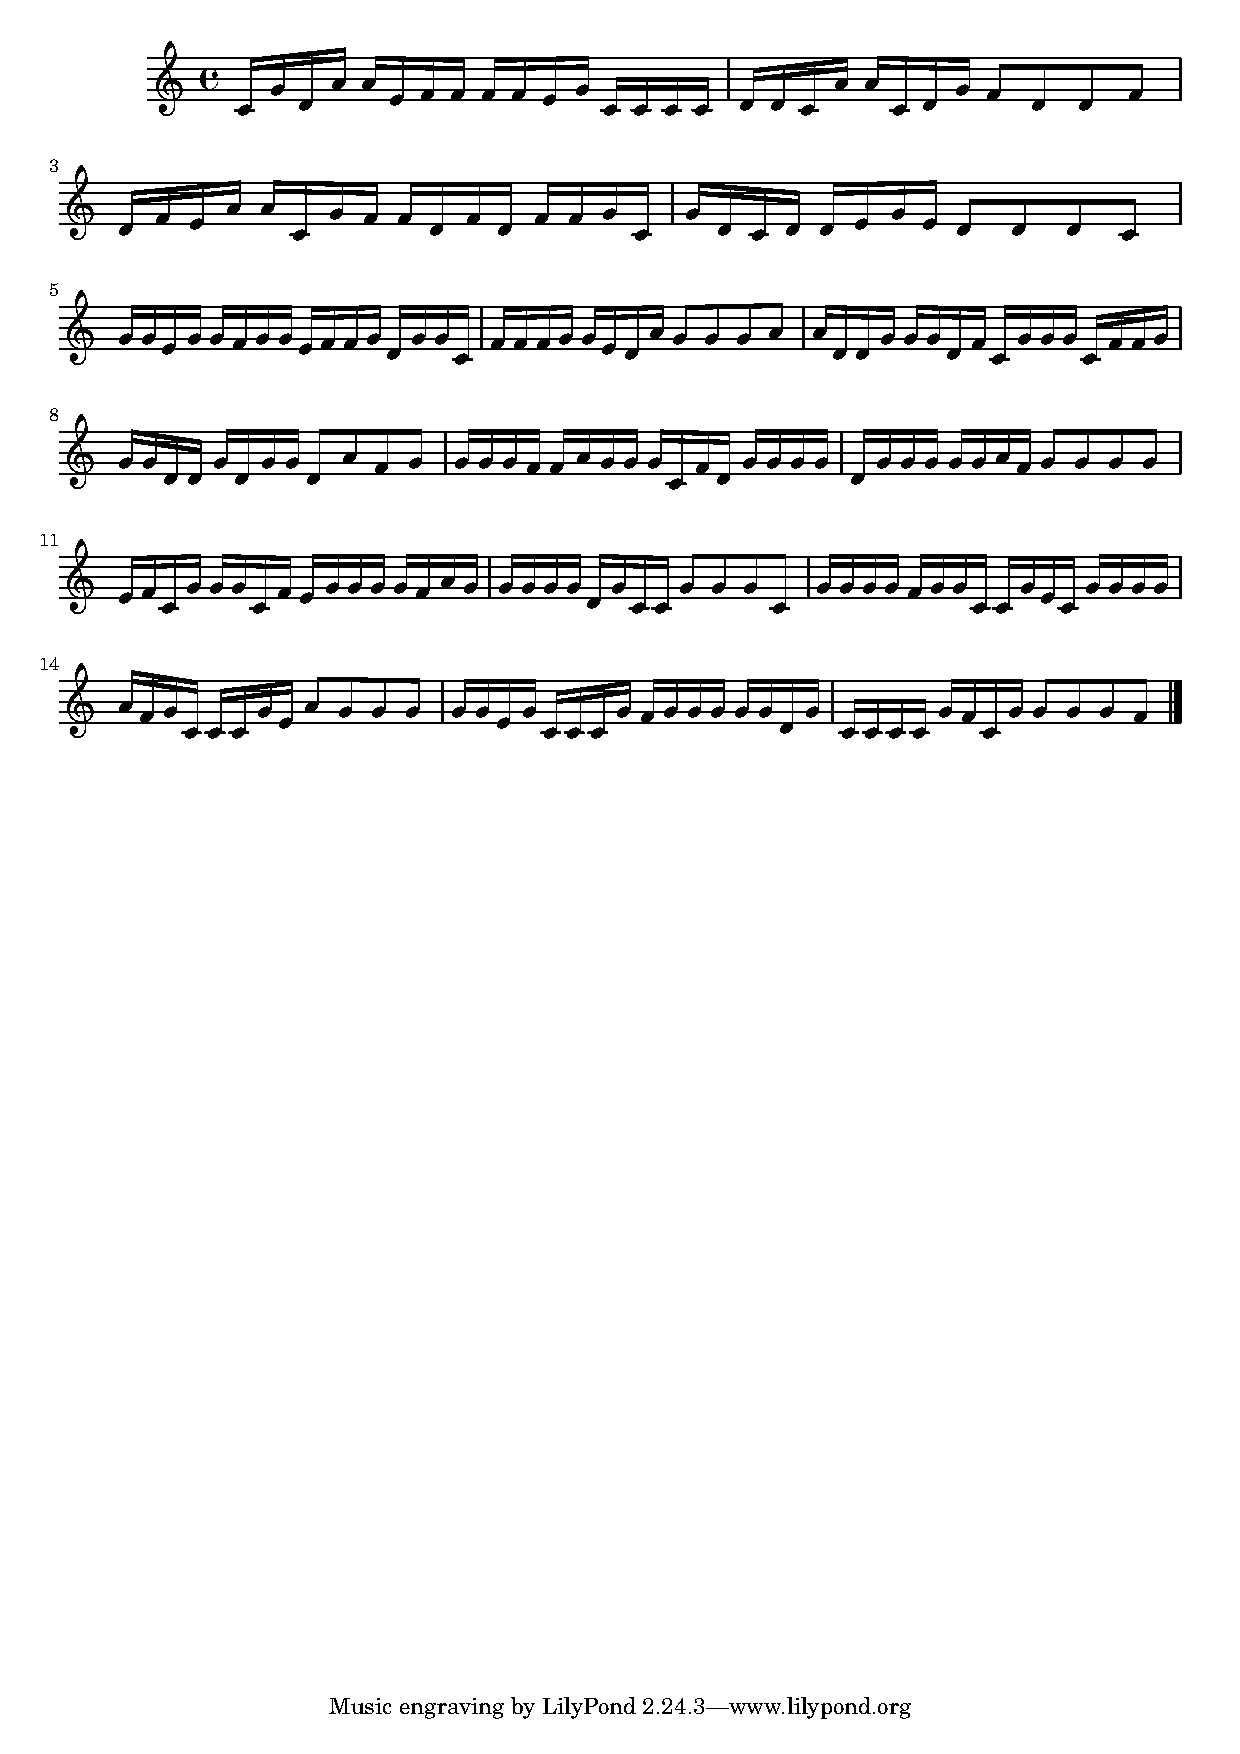
\includegraphics[trim=1cm 26.5cm 1cm 0.5cm, clip, scale=0.6]{dabby_melody_variation.pdf}
\caption{The new variation with melodic variation of Ah vous dirai-je, maman in the first 2 bars, generated by the Initial Condition $(1.01, 1, 1)$.} 
\label{fig:MVDabby}
\end{figure}

\end{document}